\documentclass[10pt, landscape]{article}
\usepackage[scaled=0.92]{helvet}
\usepackage{calc}
\usepackage{multicol}
\usepackage{ifthen}
\usepackage[a4paper,margin=3mm,landscape]{geometry}
\usepackage{amsmath,amsthm,amsfonts,amssymb}
\usepackage{color,graphicx,overpic}
\usepackage{hyperref}
\usepackage{newtxtext} 
\usepackage{enumitem}
\usepackage{amssymb}
\usepackage[table]{xcolor}
\usepackage{vwcol}
\usepackage{tikz}
\usetikzlibrary{arrows.meta}
\usetikzlibrary{calc}
\usepackage{mathtools}
\usepackage{nicematrix}
%For pictures / figures
\usepackage{color,graphicx,overpic}
\graphicspath{ {./images/midterm/} }
% for relations
\usepackage{cancel}
\usepackage{ mathrsfs }
\graphicspath{ {./images/} }
\setlist{nosep}
\usepackage{amssymb}  % For \checkmark


\pdfinfo{
  /Title (EE3408C-Midterm-Cheatsheet.pdf)
  /Creator (TeX)
  /Producer (pdfTeX 1.40.0)
  /Author (Seamus)
  /Subject (Example)
  /Keywords (pdflatex, latex,pdftex,tex)}

% Turn off header and footer
\pagestyle{empty}

\newenvironment{tightcenter}{%
  \setlength\topsep{0pt}
  \setlength\parskip{0pt}
  \begin{center}
}{%
  \end{center}
}

% redefine section commands to use less space
\makeatletter
\renewcommand{\section}{\@startsection{section}{1}{0mm}%
                                {-1ex plus -.5ex minus -.2ex}%
                                {0.5ex plus .2ex}%x
                                {\normalfont\large\bfseries}}
\renewcommand{\subsection}{\@startsection{subsection}{2}{0mm}%
                                {-1explus -.5ex minus -.2ex}%
                                {0.5ex plus .2ex}%
                                {\normalfont\normalsize\bfseries}}
\renewcommand{\subsubsection}{\@startsection{subsubsection}{3}{0mm}%
                                {-1ex plus -.5ex minus -.2ex}%
                                {1ex plus .2ex}%
                                {\normalfont\small\bfseries}}%
\renewcommand{\familydefault}{\sfdefault}
\renewcommand\rmdefault{\sfdefault}
% makes nested numbering (e.g. 1.1.1, 1.1.2, etc)
\renewcommand{\labelenumii}{\theenumii}
\renewcommand{\theenumii}{\theenumi.\arabic{enumii}.}
\renewcommand\labelitemii{•}
%  for logical not operator
\renewcommand{\lnot}{\mathord{\sim}}
\renewcommand{\bf}[1]{\textbf{#1}}
\newcommand{\abs}[1]{\vert #1 \vert}
\newcommand{\Mod}[1]{\ \mathrm{mod}\ #1}

\makeatother
\definecolor{myblue}{cmyk}{1,.72,0,.38}
\everymath\expandafter{\the\everymath \color{myblue}}
% Define BibTeX command
\def\BibTeX{{\rm B\kern-.05em{\sc i\kern-.025em b}\kern-.08em
    T\kern-.1667em\lower.7ex\hbox{E}\kern-.125emX}}
\let\iff\leftrightarrow
\let\Iff\Leftrightarrow
\let\then\rightarrow
\let\Then\Rightarrow

% Don't print section numbers
\setcounter{secnumdepth}{0}

\setlength{\parindent}{0pt}
\setlength{\parskip}{0pt plus 0.5ex}
%% this changes all items (enumerate and itemize)
\setlength{\leftmargini}{0.5cm}
\setlength{\leftmarginii}{0.5cm}
\setlist[itemize,1]{leftmargin=2mm,labelindent=1mm,labelsep=1mm}
\setlist[itemize,2]{leftmargin=4mm,labelindent=1mm,labelsep=1mm}

%My Environments
\newtheorem{example}[section]{Example}
% -----------------------------------------------------------------------

\begin{document}
\raggedright
\footnotesize
\begin{multicols}{4}


% multicol parameters
% These lengths are set only within the two main columns
\setlength{\columnseprule}{0.25pt}
\setlength{\premulticols}{1pt}
\setlength{\postmulticols}{1pt}
\setlength{\multicolsep}{1pt}
\setlength{\columnsep}{2pt}

\begin{center}
    \fbox{%
        \parbox{0.8\linewidth}{\centering \textcolor{black}{
            {\Large\textbf{EE3408C Midterm}}
            \\ \normalsize{AY26/27 sem 1}}
            \\ {\footnotesize \textcolor{myblue}{github.com/mendax1234}} 
        }%
    }
\end{center}

\section{Review of Basic MOSFETs}
\begin{enumerate}
    \item (\textbf{Triode Region}) NMOS in triode region, the drain current equation is
    $$I_D = \mu_n C_{ox} \frac{W}{L}\left[(V_{GS} - V_{TH})V_{DS} - \frac{1}{2}V_{DS}^2\right]$$
    If $V_{DS} \ll 2(V_{GS} - V_{TH})$, which is the same as $\frac{1}{2}V_{DS}^2 \ll (V_{GS} - V_{TH})V_{DS}$, the drain current equation can be simplified to
    $$I_D \approx \mu_n C_{ox} \frac{W}{L} (V_{GS} - V_{TH}) V_{DS}$$
    Thus, the NMOS behaves like a resistor and its on resistance is
    $$R_{on} = \frac{V_{DS}}{I_D} = \frac{1}{\mu_n C_{ox} \frac{W}{L} (V_{GS} - V_{TH})}$$
    For PMOS, the drain current is
    $$I_D = -\mu_p C_{ox} \frac{W}{L} \left[(V_{GS} - V_{TH})V_{DS} - \frac{1}{2}V_{DS}^2\right]$$
    \item $k_n'=\mu_nC_{OX}$ ,$V_{OV}=V_{GS}-V_{THN}$
    \item (\textbf{Saturation Region}): When NMOS operates in saturation region, its drain current is
    $$ I_D = \frac{1}{2}\mu_n C_{ox} \frac{W}{L'} (V_{GS} - V_{TH})^2$$
    For PMOS, the drain current is
    $$I_D = -\frac{1}{2}\mu_p C_{ox} \frac{W}{L'} (V_{GS} - V_{TH})^2$$
    \item (\textbf{MOSFET Operation Region Quick Check}): \\
    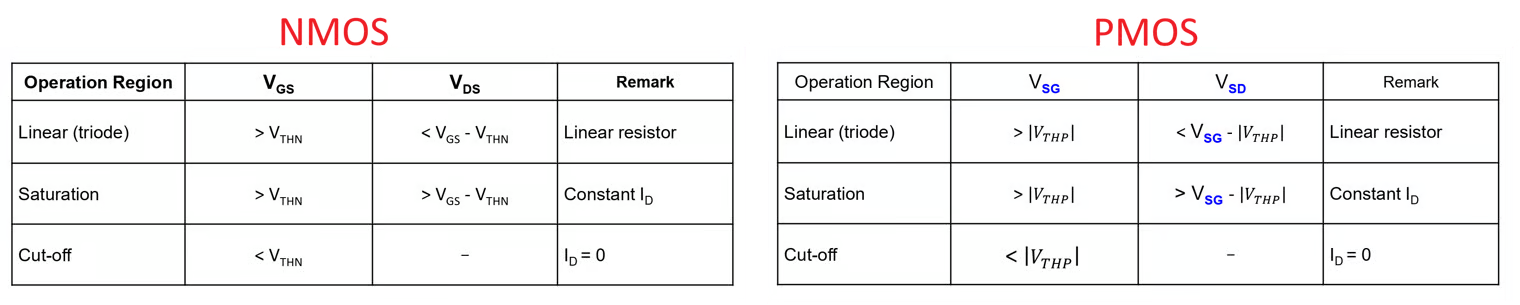
\includegraphics[width=1\linewidth]{images/midterm/1.png}
    \item (\textbf{Transconductance}): The definition of transconductance $g_m$ is given below, which holds in both saturation and linear region.
    $$g_m = \left. \frac{\partial I_D}{\partial V_{GS}} \right|_{V_{DS,\text{const.}}}$$
    For NMOS operating in \textbf{saturation region}, its $g_m$ is
    $$
    \begin{aligned}
    g_m &= \mu_n C_{ox} \frac{W}{L} (V_{GS} - V_{TH}) = \sqrt{2 \mu_n C_{ox} \frac{W}{L} I_D} \\
    &= \frac{2 I_D}{V_{GS} - V_{TH}}
    \end{aligned}
    $$
    For PMOS operating in \textbf{saturation region}, its $g_m$ is
    $$
    \begin{aligned}
    g_m &= -\mu_p C_{ox} \frac{W}{L} (V_{GS} - V_{TH}) = -\frac{2I_D}{V_{GS} - V_{TH}} \\
    &= \sqrt{2\mu_p C_{ox} \frac{W}{L} I_D}
    \end{aligned}
    $$
    For NMOS operating in \textbf{linear region}, its $g_m$ is
    $$ g_m=\mu_n C_{ox} \frac{W}{L} V_{DS}$$
    \item (\textbf{Body Effect}): In body effect, the threshold voltage for NMOS is redefined to be
    $$
    V_{TH} = V_{TH0} + \gamma \left( \sqrt{2\Phi_F + V_{SB}} - \sqrt{|2\Phi_F|} \right)
    $$
    while in PMOS, it is
    $$\vert{}V_{THp}\vert{} = \vert{}V_{TH0p}\vert{} + \gamma (\sqrt{\vert{}2\Phi_F\vert{} + V_{BS}} - \sqrt{\vert{}2\Phi_F\vert{}})$$
    For the body effect, we should understand the following 2 trends
    \begin{itemize}
        \item NMOS: $V_{SB}\uparrow \text{or } V_{BS}<0\Rightarrow V_{TH}\uparrow\Rightarrow I_D\downarrow$
        \item PMOS: $V_{BS}\uparrow \text{or } V_{BS}>0\Rightarrow |V_{THP}|\uparrow\Rightarrow I_D\downarrow$
        \item $V_{BS}=0$, no body effect.
    \end{itemize}
    \item (\textbf{Channel Length Modulation}): If the question gives $\lambda$, we should consider CLM, otherwies, don't consider. If consider CLM, the drain current when a NMOS operates in saturation region is:
    $$I_D \approx \frac{1}{2}\mu_n C_{ox}\frac{W}{L}(V_{GS}-V_{TH})^2(1+\lambda V_{DS})$$
    In EE3408C, we won't consider CLM in transconductance calculation, but \textbf{will consider that in drain current calculation} if $\lambda$ is given.
    \item Strong inversion region is usually the \textbf{same as} saturation region.
\end{enumerate}

\section{MOSFET Small-Signal Model}
\begin{enumerate}
    \item (\textbf{NMOS Small Signal Model}):
    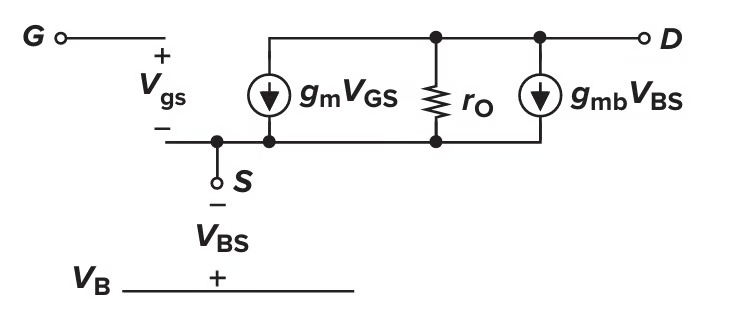
\includegraphics[width=1\linewidth]{images/midterm/2.png}
    \item (\textbf{PMOS Small Signal Model}:
    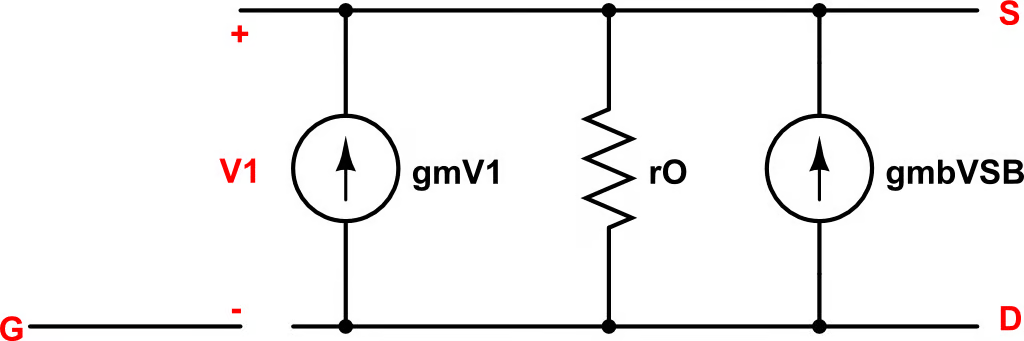
\includegraphics[width=1\linewidth]{images/midterm/3.png}
    \item In the MOS Small signal model, the output resistance only exits if we consider the CLM, and its value is $r_o\approx \frac{1}{\lambda I_D}$. Its definition formula is $r_O=\frac{\partial V_{DS}}{\partial I_D}$
    \item (\textbf{MOS Capacitance}): Define the gate-channel and overlap capacitances: $C_{GC} = WLC_{ox},C_{GS0} = C_{GD0} = C_{ov}W$
    \begin{itemize}
        \item \textbf{Cut-off region:}
        $
        C_{GS} = C_{GS0},
        C_{GD} = C_{GD0},
        C_{GB} = \frac{C_{GC}C_d}{C_{GC}+C_d}
        $
        \item \textbf{Triode region:} $C_{GC}$ is approximately equally divided between the source and drain.
        $
        C_{GS} = C_{GD} = C_{GS0} + \frac{1}{2}WLC_{ox},
        C_{GB} = 0
        $
        \item \textbf{Saturation region:} the drain side is depleted, so approximately $\frac{2}{3}C_{GC}$ appears at the source side.
        $
        C_{GS} = C_{GS0} + \frac{2}{3}WLC_{ox},
        C_{GD} = C_{GD0},
        C_{GB} = 0
        $
    \end{itemize}
    \item \textbf{Miscs}
    \begin{itemize}
        \item When the question asks how one thing changes with the other thing, we do \textbf{partial differentiation} to find the change rate using the given values!
    \end{itemize}
\end{enumerate}

\section{Single-Stage Amplifier Design}
\begin{enumerate}
    \item Common MOSFET impedance: \\
    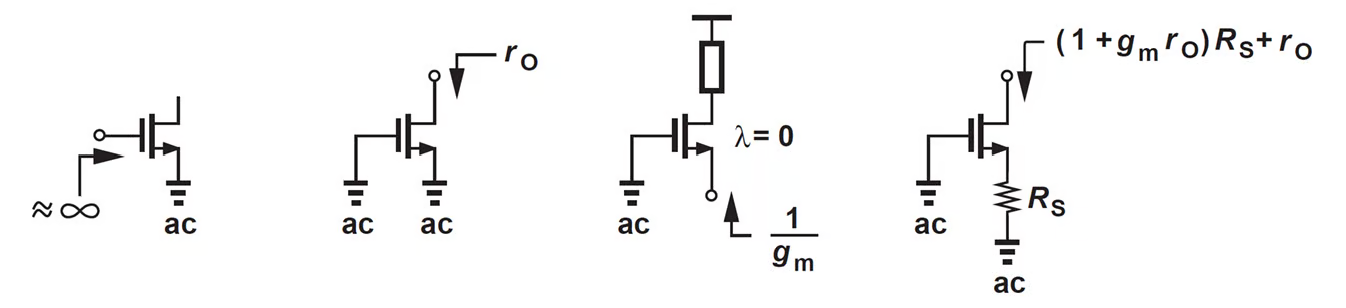
\includegraphics[width=1\linewidth]{images/midterm/4.png}
    \begin{itemize}
        \item In the third case, no matter what is connected at the drain, the resistance looking from the source terminal is always $\frac{1}{g_m}$
        \item For a diode-connected MOSFET (gate and drain are connected together), its impedance is always $\frac{1}{g_m}$ (from both the view of source and drain) if we ignore the body effect.
    \end{itemize}
    \item Common transconductance in the circuit level:
    \begin{itemize}
        \item In a single-stage CS amplifier where the input is at the \textbf{gate} terminal and the output is at the \textbf{drain} terminal of the NMOS M1, $G_m=g_{m1}$.
        \item In a single-stage CD amplifier (Source follower) where the input is at the \textbf{gate} terminal and the output is at the \textbf{source} terminal of the NMOS M1, $G_m=g_{m1}$.
        \item In a single-stage CG amplifier where the input is at the \textbf{source} terminal and the output is at the \textbf{drain} terminal of teh NMOS M1, $G_m=-g_{m1}$.
        \item In a cascode stage amplifier, basically 2-stage amplifier (CS + CG), we usually calculate the final $G_m$ by separating the stage \\
        \begin{center}
            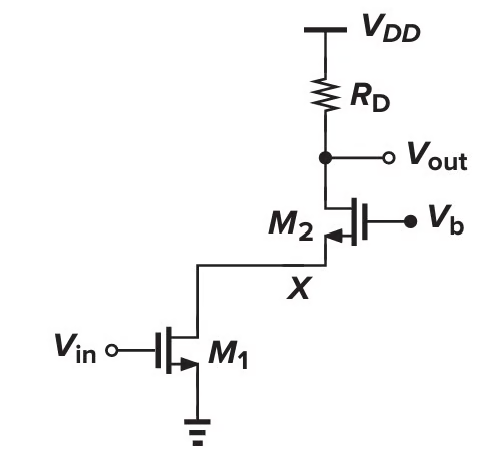
\includegraphics[width=0.5\linewidth]{images/midterm/5.png}
        \end{center}
        So, $G_m=\frac{i_{out}}{v_{in}}=\frac{i_{out}}{v_{x}}\times\frac{v_{x}}{v_{in}}$. And we can use the similar method to find the voltage gain of the first-stage and use our faster conclusions to find the $G_m'$ of the second stage. Thus, find the $G_m$ of the whole stage! As a shortcut, if the output is connect to drain terminal of NMOS M2, $G_m=g_{m1}$
    \end{itemize}
    \item Intuitive Understanding of each type of amplifier:
    \begin{itemize}
        \item The CS amplifier is used to amplify the input signal, but in an \textbf{inverting} manner.
        \item The CD amplifier (source follower) is used to pass the voltage at its input to its output with small loss, thus its $A_v\approx 1$.
        \item The CG amplifier is used to \textbf{amplify the input signal} (or provide \textbf{low input resistance}) while producing a non-inverted voltage output.
        \item The cascode amplifier combines a \textbf{CS stage and a CG stage}: the CS transistor converts the input voltage into a signal current, while the CG transistor keeps the CS transistor's drain voltage relatively constant. Thus, it provides \textbf{high voltage gain} by achieving a large output resistance while retaining the transconductance of the CS stage.
    \end{itemize}
\end{enumerate}

\section{Frequency Response}
\begin{enumerate}
    \item (\textbf{Bode Plot}): When drawing the magnitude and phase bode plot, it suffices to just write the transfer function in the $s$ form and then determine the poles and zeros (origin or left or right) and then use the summary to draw the magnitude and phase bode plot.
    \item (\textbf{Miller Theorem}): In the following circuit, $C_1=1-A_v$ and $C_2=C(1-\frac{1}{A_v})$ \\
    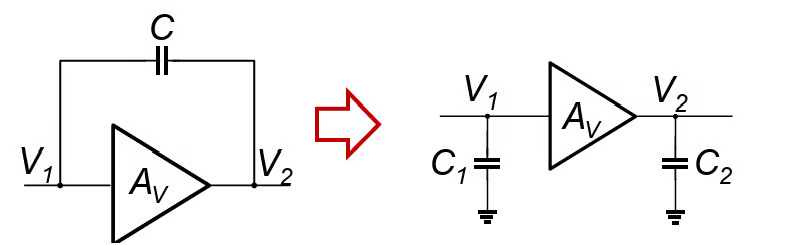
\includegraphics[width=1\linewidth]{images/midterm/6.png}
    \item (\textbf{Association of Poles}):
    \begin{itemize}
        \item When using the rule of association of poles, it suffices if we just draw the circuit diagram like below (not necessarily the small-signal circuit): \\
        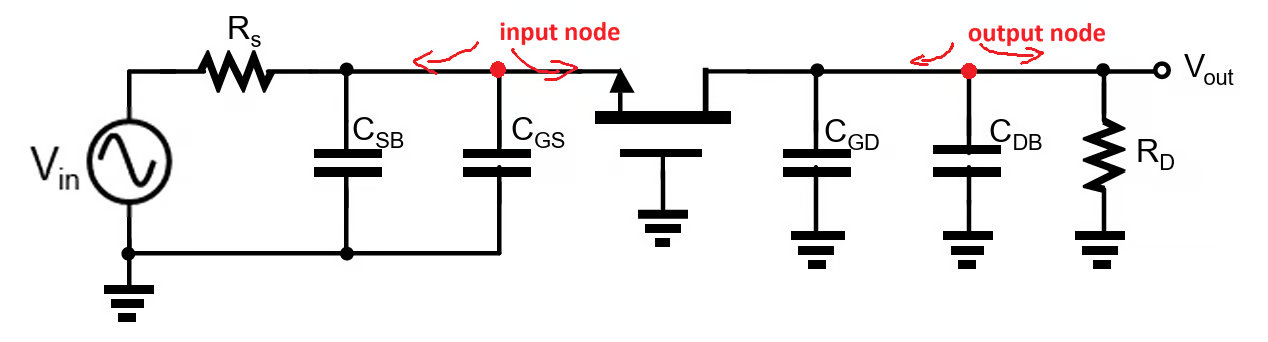
\includegraphics[width=1\linewidth]{images/midterm/7.png}
        \item When constructing a diagram as such, we treat $V_{DD}$ and $V_{in}$ as AC ground.
        \item As in EE3408C, we are only dealing with circuits with positive impedance, the rule of \textbf{association of poles} always give us \textbf{LHP}!
    \end{itemize}
    \item (\textbf{Shortcut to find zeros}):
    \begin{itemize}
        \item When finding the value of zeros, we should draw the small-signal diagram as follows to find the value for the \textbf{high-frequency zero}: \\
        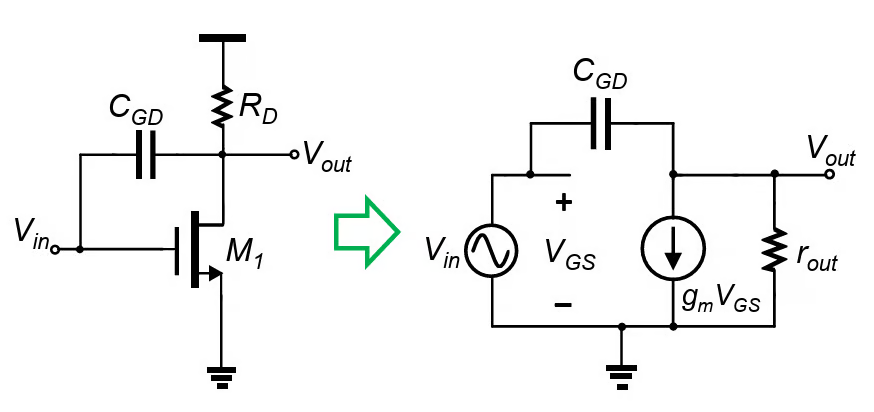
\includegraphics[width=1\linewidth]{images/midterm/8.png}
    \end{itemize}
    \item In a multiple-pole system, the \textbf{dominant pole} is the pole with the lowest pole frequency.
    \item From pole frequency $\omega$ to actual frequency $f$, $f=\frac{\omega}{2\pi}$
    \item \textbf{Unit Table}: \\
    \begin{center}
        \begin{tabular}{c|c|c}
            \textbf{Factor} & \textbf{Name} & \textbf{Symbol} \\ \hline
            $10^{9}$   & Giga  & G \\
            $10^{6}$   & Mega  & M \\
            $10^{3}$   & Kilo  & k \\
            $10^{2}$   & Hecto & h \\
            $10^{1}$   & Deca  & da \\
            $10^{-1}$  & Deci  & d \\
            $10^{-2}$  & Centi & c \\
            $10^{-3}$  & Milli & m \\
            $10^{-6}$  & Micro & $\mu$ \\
            $10^{-9}$  & Nano  & n \\
            $10^{-12}$ & Pico  & p \\
            $10^{-15}$ & Femto & f \\
            $10^{-18}$ & Atto  & a \\
            $10^{-21}$ & Zepto & z
        \end{tabular}
    \end{center}

\end{enumerate}

\end{multicols}

% Dividing Line
% \hrulefill \\
% \begin{multicols}{4}
% \begin{enumerate}
% \end{enumerate}
% \end{multicols}

\end{document}